%%
% 第三章 天基网络可信协同计算卸载场景与基础建模
%%

\chapter{天基网络可信协同计算卸载场景与基础建模}
\label{chap:ch3_unified_model}

\section{引言}
\label{sec:ch3_intro}

天基网络协同计算卸载的主要挑战不仅仅是技术优化，而是如何应对动态拓扑、异构资源与可信协同之间的复杂约束。卫星轨道的运动使得星间与星地链路的可达性、带宽以及可见窗口不断变化，网络拓扑表现出强烈的时变特性。此外，卫星终端、卫星边缘节点以及地面控制中心在计算能力、存储容量、能量预算和通信条件上存在显著差异，无法采用静态的集中式调度模型。

协同卸载是一个由多个节点参与的分布式过程，网络中缺乏稳定且持续可达的中心节点，节点状态上报存在延迟、失真甚至虚假报告的问题，任务执行的结果和协同行为需要具备可信的追溯机制。因此，天基网络协同计算卸载不仅要解决资源匹配和任务分配，还需要在拓扑动态性、资源异构性和状态可信性之间建立统一的建模框架。

目前，已有研究多从单一角度处理上述问题。计算卸载相关研究通常采用简化的节点与链路假设，重点关注时延与能耗优化，对节点状态可信共享、任务执行追溯以及长期协作激励考虑不足；面向多时间尺度的研究则往往分别讨论系统层长期协同与任务层即时决策，尚未充分刻画二者在同一方法体系中的层次衔接关系。若协同资源分配、可信状态共享与任务卸载决策分别采用彼此独立的符号体系和建模假设，则系统层协同结果难以自然转化为任务层约束，任务层执行反馈也难以回流至系统层状态更新。因此，在具体方法展开之前，有必要建立涵盖网络拓扑、节点资源、任务属性、链路传输、执行代价以及区块链可信控制平面结构和状态摘要的统一基础模型，为后续章节的状态构造、代价计算与目标函数设计奠定一致的形式化基础。

为此，本章在第\ref{chap:ch4_system_resource_allocation}章和第\ref{chap:ch5_task_offloading}章的具体方法设计之前，首先给出统一的天基网络协同计算卸载场景描述与基础建模。具体来说，本章的目标有两方面：一方面，描绘由卫星终端、卫星边缘节点、地面控制中心和区块链可信控制平面共同组成的协同计算卸载场景，明确参与角色、任务生命周期流程与基本运行框架；另一方面，建立一个统一的符号体系，涵盖网络拓扑、节点资源、任务属性、链路传输、本地计算、星间卸载、能耗开销、联盟链结构与链上状态摘要等基础模型，为后续章节中的代价计算、状态构造与目标函数设计提供共同的形式化基础。

\section{天基网络可信协同计算卸载场景}
\label{sec:ch3_scenario}
\label{subsec:ch3_blockchain_role}

本节首先给出本文所研究的协同计算卸载场景。整个场景由物理网络层和区块链可信控制平面共同支撑：物理网络层提供节点之间动态时变的星间与星地链路，是任务执行与数据传输的物理载体；区块链可信控制平面以联盟链与智能合约为载体，承载节点状态摘要、任务生命周期事件、节点信誉演化与模型版本凭据等可信公共信息。参与协同计算的实体进一步划分为卫星终端、卫星边缘节点、地面控制中心和区块链可信控制平面四类角色，并在其上协同完成由``任务生成—状态感知—候选节点筛选—卸载决策—任务执行—结果反馈—链上更新''七个阶段构成的任务生命周期流程。场景的总体结构如图\ref{fig:ch3_scenario_overview}所示。

\begin{figure}[htbp]
    \centering
    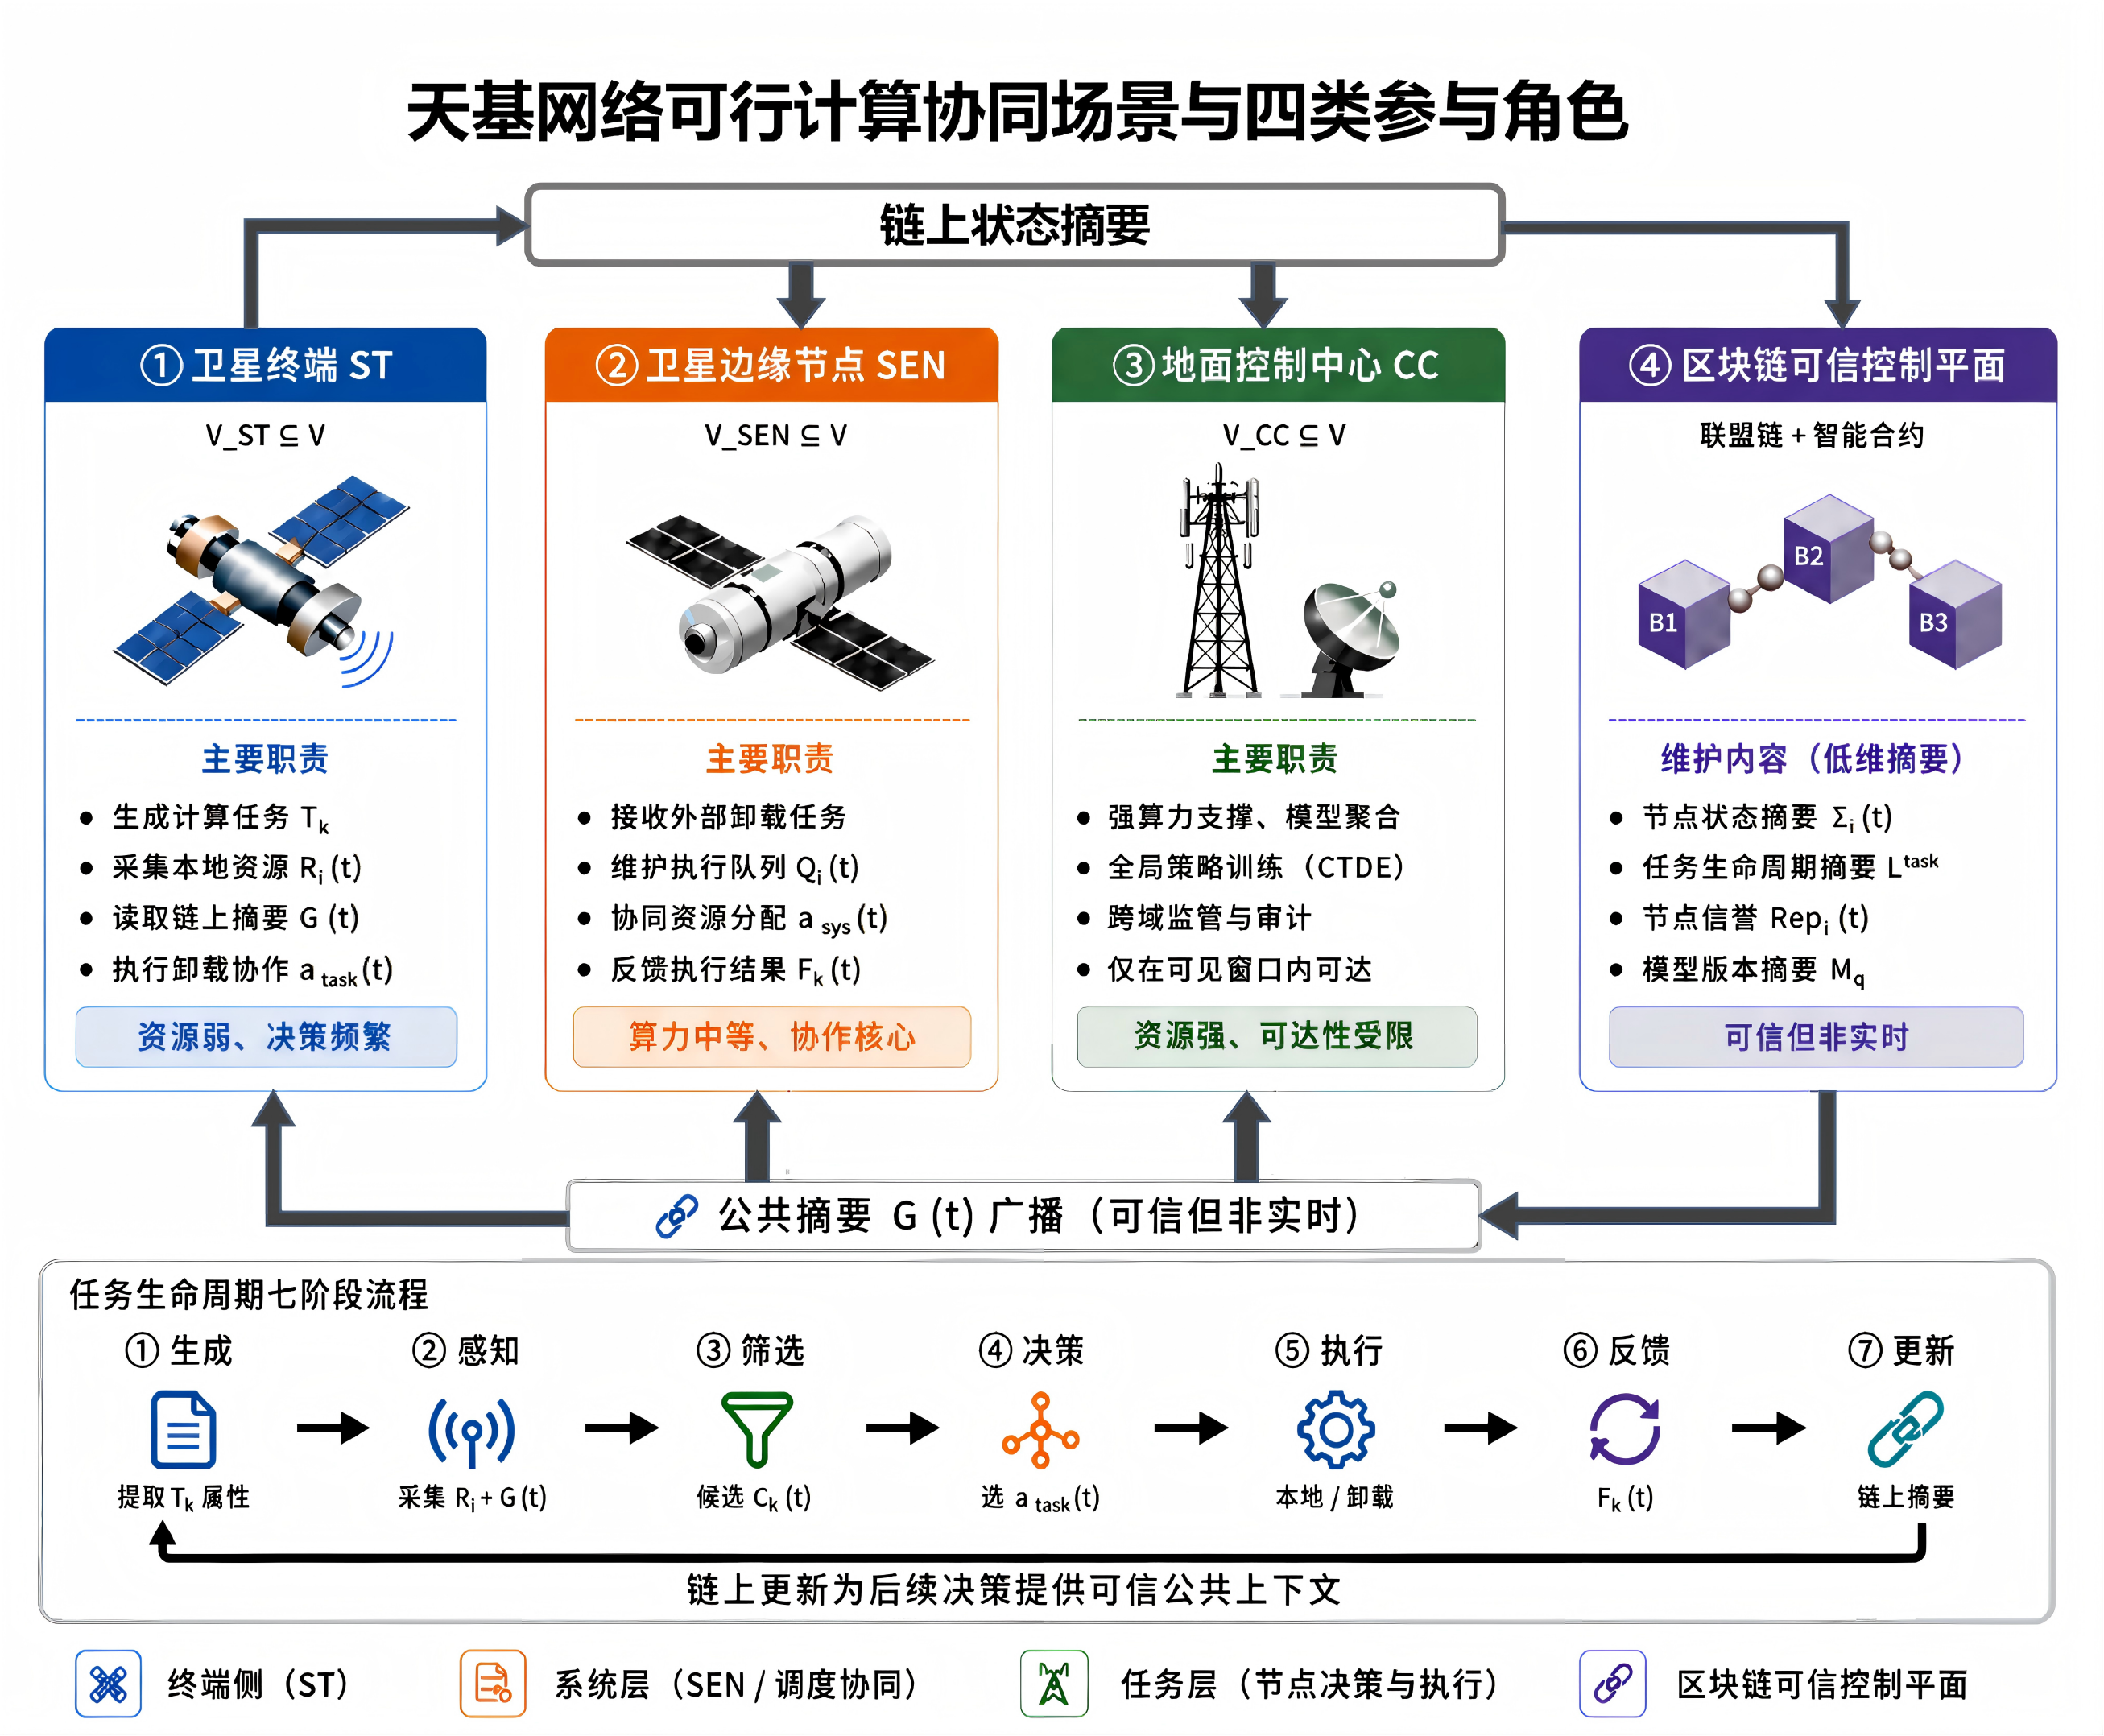
\includegraphics[width=0.96\textwidth]{figures/new3-2.png}
    \caption{天基网络可信协同计算卸载场景与四类参与角色}
    \label{fig:ch3_scenario_overview}
\end{figure}

图\ref{fig:ch3_scenario_overview}从上至下展示了天基网络可信协同计算卸载场景的三类要素：物理网络层、四类参与角色与任务生命周期流程。

物理网络层刻画卫星轨道运动以及由此产生的时变星间和星地链路。链路的可达性、可用带宽和可见窗口随轨道相对几何关系动态变化，使节点之间的状态广播频率和传输能力同样具有时变特性。节点本地状态摘要 $\Sigma_i(t)$ 在频次受控的前提下经此层链路上链，其上链频率综合考虑链路带宽预算、可见窗口长度和共识开销三方面约束，避免因高频上链而挤占任务数据通信带宽；具体的网络拓扑模型与链路状态向量将在第\ref{subsec:ch3_topology_model}节形式化给出。

天基网络可信协同计算卸载场景主要有四类参与角色，分别承担不同的协同职责。卫星终端 ST（属于 $\mathcal{V}_{\mathrm{ST}}$）一般指资源受限的小型卫星或专用终端，其特点是计算与能量资源相对薄弱、决策频繁，主要负责生成计算任务、采集本地资源状态、读取链上公共摘要并执行卸载动作，是任务发起方；卫星边缘节点 SEN（属于 $\mathcal{V}_{\mathrm{SEN}}$）通常为具备较强算力与转发能力的卫星平台，是协作执行的核心，负责接收外部卸载任务、维护执行队列、参与协同资源分配并向链上反馈执行结果；地面控制中心 CC（属于 $\mathcal{V}_{\mathrm{CC}}$）资源最为充裕，但其与天基节点之间的可达性受限于轨道可见窗口，主要承担强算力支持、模型聚合、全局策略训练以及跨域监管与审计等职责；区块链可信控制平面以联盟链与智能合约为载体，本身不直接参与高频任务执行，而是作为可信状态共享与治理底座，维护节点状态摘要、任务生命周期事件、节点信誉评分与模型版本摘要等低维可信信息，并通过公共摘要向前三类角色统一广播。

形式化地，参与协同计算的节点集合可表示为
\begin{equation}
    \mathcal{V}=\mathcal{V}_{\mathrm{ST}}\cup\mathcal{V}_{\mathrm{SEN}}\cup\mathcal{V}_{\mathrm{CC}}.
    \label{eq:ch3_node_set}
\end{equation}
任一物理节点既可能是任务发起方，也可能是任务执行方，但不同节点在算力、存储、能量和链路条件上存在显著差异。为支撑后续可信状态共享建模，本文进一步从功能职责角度定义共识维护节点集合 $\mathcal{V}_{\mathrm{con}}\subseteq\mathcal{V}$、任务执行节点集合 $\mathcal{V}_{\mathrm{exe}}\subseteq\mathcal{V}$ 和链下存储节点集合 $\mathcal{V}_{\mathrm{sto}}\subseteq\mathcal{V}$。三类集合分别对应区块定序与状态摘要广播、任务承接与执行反馈、以及大规模实体对象的链下存储。需要说明的是，这里的 $\mathcal{V}_{\mathrm{exe}}$ 表示物理意义上的任务执行能力集合，并不等同于联盟链网络中的非共识账本节点；同一物理节点可同时承担多种功能职责，例如核心 SEN 可同时参与共识和任务执行，CC 在可见窗口内也可兼具共识、执行和链下存储能力。因此，$\mathcal{V}_{\mathrm{con}}$、$\mathcal{V}_{\mathrm{exe}}$ 与 $\mathcal{V}_{\mathrm{sto}}$ 之间允许存在交集。

任务生命周期七阶段流程刻画了一次具体协同计算从发起到完成所经历的关键阶段。生成：卫星终端产生计算任务并提取 $T_k=(s_k,c_k,d_k,\tau_k,\zeta_k,t_k^{\mathrm{arr}})$ 等任务属性；感知：终端采集本地资源状态 $R_i(t)$ 与链上公共摘要 $G(t)$，形成``本地观测+链上摘要''的复合状态视图；筛选：基于链路可见窗口、节点信誉门限与负载约束确定可卸载候选节点集合 $\mathcal{N}_k^{\mathrm{off}}(t)$，并与本地节点共同构成任务动作集合 $\mathcal{A}_k(t)$；决策：在 $\mathcal{A}_k(t)$ 上根据时延、能耗与并发开销估计选择本地执行或卸载动作 $a_{\mathrm{task}}(t)$；执行：目标节点（本地或卸载节点）完成任务计算与结果回传；反馈：系统记录任务完成时延、能耗、成功状态和异常事件，封装为反馈向量 $F_k(t)$；更新：反馈摘要写入链上，进而更新节点信誉、负载摘要与模型版本统计，并以``链上更新驱动下一轮决策''的方式形成持续演化。

由上述阶段可见，协同计算卸载并不是简单的``任务发起—节点选择—执行返回''的单向调用，而是由感知、决策、执行、反馈和更新共同支撑的持续过程：状态感知与链上更新提供可信公共上下文，候选节点筛选与卸载决策由后续章节中的系统层和任务层方法分别承担，任务执行结果则通过链上事件回流为后续策略迭代提供依据。关于该过程在不同时间尺度下的形式化描述以及两层方法之间的耦合机制，将在第\ref{chap:ch4_system_resource_allocation}章和第\ref{chap:ch5_task_offloading}章中分别给出。

图\ref{fig:ch3_scenario_overview}最右侧的区块链可信控制平面被本文定位为``可信但非实时''的状态共享与治理底座。这一定位包含两层含义。其一，该控制平面不直接替代实时调度器，亦不存储高维原始任务数据，而是仅维护协同所需的低维可信信息：通过摘要上链与实体链下存储相结合的方式，为系统层协同资源分配提供可信公共状态、为任务层卸载决策提供候选节点摘要与模型版本凭据，并通过任务执行结果回流更新节点信誉与系统状态；具体的联盟链网络组成、区块结构以及链上状态摘要的形式化定义将在第\ref{subsec:ch3_chain_structure}节与第\ref{subsec:ch3_state_summary}节给出，而节点信誉演化、任务生命周期存证和模型版本可信维护等动态治理机制由于与下游方法的状态空间和奖励设计紧密耦合，将在第\ref{chap:ch4_system_resource_allocation}章和第\ref{chap:ch5_task_offloading}章中分别展开。其二，``非实时''是指区块链共识、广播与验证的总附加时延 $D_{\mathrm{chain}}$ 通常处于亚秒至数秒量级。由于系统层多节点资源协同关注较长时间尺度上的负载演化与信誉积累，而任务层卸载决策受任务到达瞬间的链路窗口与队列状态约束，$D_{\mathrm{chain}}$ 在系统层尺度上可被视为可容忍的小量，但在任务层尺度上不可忽略。具体的时间尺度划分以及链上摘要在不同方法中的嵌入方式，将在第\ref{chap:ch4_system_resource_allocation}章和第\ref{chap:ch5_task_offloading}章中结合各自方法的决策粒度分别给出。

\section{系统基础模型}
\label{sec:ch3_basic_model}

本节按照``物理资源—任务与代价—可信控制''的逻辑展开，建立后续章节共用的符号体系。其中，第\ref{subsec:ch3_topology_model}节至第\ref{subsec:ch3_exec_model}节刻画 ST/SEN/CC 三类计算节点的物理属性与执行代价，第\ref{subsec:ch3_chain_structure}节至第\ref{subsec:ch3_state_summary}节刻画区块链可信控制平面的结构组成与状态摘要。各子模型在完成形式化定义后，进一步说明其与系统层协同资源分配和任务层实时卸载决策之间的层次关系，以保证全文建模假设、变量含义和方法展开的一致性。

\subsection{网络拓扑模型}
\label{subsec:ch3_topology_model}

天基网络拓扑随轨道运动和链路可见关系动态变化。本文将其表示为时变有向图
\begin{equation}
    \mathcal{G}(t)=\big(\mathcal{V},\mathcal{E}_{\mathrm{link}}(t)\big),
    \label{eq:ch3_dynamic_graph}
\end{equation}
其中，$\mathcal{V}$ 由式\eqref{eq:ch3_node_set}给出，$\mathcal{E}_{\mathrm{link}}(t)$ 为时刻 $t$ 可用通信链路集合。若节点 $i$ 与节点 $j$ 在时刻 $t$ 存在可用链路，则 $(i,j)\in\mathcal{E}_{\mathrm{link}}(t)$。链路状态可表示为
\begin{equation}
    \ell_{ij}(t)=\big(B_{ij}(t),d_{ij}^{\mathrm{prop}}(t),\tau_{ij}^{\mathrm{vis}}(t),p_{ij}^{\mathrm{loss}}(t)\big),
    \label{eq:ch3_link_state}
\end{equation}
其中，$B_{ij}(t)$ 为可用带宽，$d_{ij}^{\mathrm{prop}}(t)$ 为传播时延，$\tau_{ij}^{\mathrm{vis}}(t)$ 为剩余可见窗口，$p_{ij}^{\mathrm{loss}}(t)$ 为链路中断概率估计。

上述拓扑与链路状态定义给出了节点间协同关系的物理可行域。在系统层协同资源分配中，$\ell_{ij}(t)$ 可被进一步聚合为链路统计特征，用以刻画节点之间长期协作的稳定性与可达性；在任务层实时卸载决策中，$\tau_{ij}^{\mathrm{vis}}(t)$ 则构成候选节点筛选的重要约束，决定当前任务是否能够在链路可见窗口内完成传输与返回。

\subsection{节点资源模型}
\label{subsec:ch3_resource_model}

节点 $v_i$ 的资源状态定义为
\begin{equation}
    R_i(t)=\big(F_i(t),M_i(t),Q_i(t),E_i(t),\rho_i(t),\mathrm{Rep}_i(t)\big),
    \label{eq:ch3_resource_state}
\end{equation}
其中，$F_i(t)$ 表示可用计算能力，$M_i(t)$ 表示可用存储或缓存容量，$Q_i(t)$ 表示任务队列长度，$E_i(t)$ 表示剩余能量或能量预算，$\rho_i(t)$ 表示资源利用率，$\mathrm{Rep}_i(t)$ 表示节点信誉评分。资源状态在每个决策周期由节点本地采样获得，再经摘要化处理后上链共享，其摘要形式将在第\ref{subsec:ch3_state_summary}节给出；信誉评分 $\mathrm{Rep}_i(t)$ 的具体演化规则将在第\ref{chap:ch4_system_resource_allocation}章第\ref{subsec:ch4_reward_design}节中结合系统层奖励函数设计给出。

基于上述资源状态表示，后续章节可在不同时间尺度下选取相应状态分量。第\ref{chap:ch4_system_resource_allocation}章面向窗口级协同，将 $R_i(t)$ 投影为节点局部观测 $l_t^i$，以刻画节点长期负载与协作能力；第\ref{chap:ch5_task_offloading}章面向单任务到达瞬间的实时决策，则从中抽取队列长度、剩余能量和资源利用率等局部状态，形成任务层状态 $\bm{x}^{\mathrm{local}}$。

\subsection{任务模型}
\label{subsec:ch3_task_model}

设任务集合为 $\mathcal{T}$。任一任务 $T_k$ 可表示为
\begin{equation}
    T_k=\big(s_k,c_k,d_k,\tau_k,\zeta_k,t_k^{\mathrm{arr}}\big),
    \label{eq:ch3_task_model}
\end{equation}
其中，$s_k$ 为任务输入数据规模，$c_k$ 为完成任务所需的 CPU 周期数，$d_k$ 为任务最大可接受完成时延，$\tau_k$ 为任务类型标识，$\zeta_k$ 为任务优先级，$t_k^{\mathrm{arr}}$ 为任务到达时间。该表示方式既适用于遥感图像识别、目标检测等智能推理任务，也适用于通信解调、数据压缩和信号处理等传统计算任务。后文所有与链路可见窗口有关的约束均采用时延量 $D_{k,ij}^{\mathrm{tx}}(t)$ 或任务截止时延 $d_k$ 表示，$\tau_k$ 仅作为任务类型标识使用。

为使建模具有典型物理锚点，本文以低轨遥感星座辅助应急图像识别任务作为参考场景：考虑由若干卫星终端、卫星边缘节点和地面控制中心构成的协同计算网络，单次试验典型时长为分钟级，单任务典型输入数据规模为兆字节量级，典型计算量为百万至十亿浮点运算量级。第\ref{chap:ch4_system_resource_allocation}章和第\ref{chap:ch5_task_offloading}章的实验将分别在该场景下，按照系统层和任务层不同时间尺度展开。

在后续两章中，任务模型对应不同粒度的状态刻画。第\ref{chap:ch4_system_resource_allocation}章关注统计窗口内任务负载的整体演化，因此将 $\mathcal{T}$ 中任务类型、计算量和截止期等信息聚合为任务分布摘要 $D^{\mathrm{task}}(t)$；第\ref{chap:ch5_task_offloading}章关注单任务到达时的即时动作选择，因此将 $T_k$ 的输入规模、计算量、时延约束、任务类型和优先级组织为任务特征向量 $\bm{x}^{\mathrm{task}}$。

\subsection{链路传输模型}
\label{subsec:ch3_tx_model}

当任务 $T_k$ 从节点 $i$ 卸载至节点 $j$ 时，其传输速率可写为
\begin{equation}
    R_{ij}(t)=B_{ij}(t)\log_2\!\left(1+\frac{P_i h_{ij}(t)}{N_0 B_{ij}(t)}\right),
    \label{eq:ch3_rate_model}
\end{equation}
其中，$P_i$ 为节点 $i$ 的发送功率，$h_{ij}(t)$ 为信道增益，$N_0$ 为噪声功率谱密度。相应传输时延为
\begin{equation}
    D_{k,ij}^{\mathrm{tx}}(t)=\frac{s_k}{R_{ij}(t)}+d_{ij}^{\mathrm{prop}}(t).
    \label{eq:ch3_tx_delay}
\end{equation}

式\eqref{eq:ch3_rate_model}和式\eqref{eq:ch3_tx_delay}刻画了任务跨节点传输的基本时延构成。第\ref{chap:ch5_task_offloading}章将在任务层采用 $L_i^{\mathrm{off}}(n,t)$ 表示卸载至候选节点 $n$ 时的端到端完成时延，其中上行传输时延由式\eqref{eq:ch3_tx_delay}给出。为区分基础链路时延与任务层端到端时延，本文在本章采用 $D$ 表示基础时延量，在第\ref{chap:ch5_task_offloading}章采用 $L$ 表示任务完成时延，两者在物理含义上相互一致，在建模粒度上有所区别。

\subsection{本地计算与星间卸载模型}
\label{subsec:ch3_exec_model}

若任务在本地执行，其完成时延为
\begin{equation}
    D_{k,i}^{\mathrm{loc}}(t)=W_i(t)+\frac{c_k}{f_{k,i}^{\mathrm{alloc}}(t)},
    \label{eq:ch3_local_compute_delay}
\end{equation}
其中，$W_i(t)$ 为排队等待时延，$f_{k,i}^{\mathrm{alloc}}(t)$ 为节点 $i$ 分配给任务 $T_k$ 的有效计算频率。若任务卸载至节点 $j$ 执行，其完成时延为
\begin{equation}
    D_{k,ij}^{\mathrm{off}}(t)=D_{k,ij}^{\mathrm{tx}}(t)+W_j(t)+\frac{c_k}{f_{k,j}^{\mathrm{alloc}}(t)}+\Delta_{k,j}^{\mathrm{conc}}(t),
    \label{eq:ch3_offload_delay_unified}
\end{equation}
其中，$\Delta_{k,j}^{\mathrm{conc}}(t)$ 表示多任务并发引起的额外开销，既包括新任务自身完成时延的增加，也包括新任务加入后对目标节点存量任务剩余完成时间的影响。该项体现了任务层卸载决策中资源竞争与任务耦合的关键因素，第\ref{chap:ch5_task_offloading}章将进一步对其进行形式化分解与近似刻画。为减少符号负担，第\ref{chap:ch5_task_offloading}章在单任务视角下将 $\Delta_{k,j}^{\mathrm{conc}}(t)$ 记为 $\Delta_i(n,t)$，其中 $i$ 表示新到达任务，$n$ 表示候选目标节点；并将其完整形式化定义记为 $CO_i(n,t)$，预测估计记为 $\widehat{\Delta}_i(n,t)$，各分量含义均与本章保持一致。

本地执行能耗可近似表示为
\begin{equation}
    E_{k,i}^{\mathrm{loc}}(t)=\kappa_i c_k\big(f_{k,i}^{\mathrm{alloc}}(t)\big)^2,
    \label{eq:ch3_local_energy_unified}
\end{equation}
其中，$\kappa_i$ 为节点 $i$ 的有效电容系数。卸载执行能耗可表示为
\begin{equation}
    E_{k,ij}^{\mathrm{off}}(t)=P_i \frac{s_k}{R_{ij}(t)}+\kappa_j c_k\big(f_{k,j}^{\mathrm{alloc}}(t)\big)^2+E_{k,ij}^{\mathrm{wait}}(t),
    \label{eq:ch3_offload_energy_unified}
\end{equation}
其中，$E_{k,ij}^{\mathrm{wait}}(t)$ 表示等待和连接维持过程中的额外能耗。

上述本地执行与卸载执行模型构成全文统一的代价刻画基础。第\ref{chap:ch4_system_resource_allocation}章将在统计窗口内聚合相应时延与能耗项，以形成系统层奖励函数中的效率评价；第\ref{chap:ch5_task_offloading}章则在单任务粒度上进一步展开等待能耗、边缘侧执行能耗折算和并发扰动项，并据此构造任务层综合代价 $J_i(a_t)$。因此，后续章节中能耗项的具体展开可理解为对本章基础代价模型的时间尺度细化，而非另行引入新的物理代价假设。

\subsection{联盟链结构与区块结构}
\label{subsec:ch3_chain_structure}

考虑到天基协同计算环境中节点身份相对受控、共识效率约束严格、不同业务事件之间存在频次与时效差异，本文采用联盟链方式组织区块链可信控制平面，并对其网络结构、链上链下数据划分以及区块结构进行形式化描述。本小节给出联盟链的结构性定义，而具体的事件写入、共识流程以及节点信誉演化、任务生命周期存证、模型版本治理等动态机制将在下游章节结合方法流程展开。

\subsubsection{联盟链网络组成}

设区块链网络由一组授权账本节点 $\mathcal{V}_{\mathrm{chain}}\subseteq\mathcal{V}$ 构成。按照账本维护权限，可将其划分为共识节点集合 $\mathcal{V}_{\mathrm{con}}$ 和账本接入节点集合 $\mathcal{V}_{\mathrm{cli}}$。其中，$\mathcal{V}_{\mathrm{con}}$ 负责区块定序、交易校验与状态广播，是账本一致性的直接维护方；$\mathcal{V}_{\mathrm{cli}}$ 不参与区块生成，但可进行状态读取、事件提交与本地校验。二者满足 $\mathcal{V}_{\mathrm{con}}\cap\mathcal{V}_{\mathrm{cli}}=\varnothing$ 且 $\mathcal{V}_{\mathrm{con}}\cup\mathcal{V}_{\mathrm{cli}}=\mathcal{V}_{\mathrm{chain}}$。需要强调的是，$\mathcal{V}_{\mathrm{cli}}$ 仅表示联盟链中的账本访问身份，与前文定义的任务执行节点集合 $\mathcal{V}_{\mathrm{exe}}$ 属于不同维度，二者不构成排斥关系。考虑到原始任务输入、完整模型参数和详细执行日志在体量上显著高于状态摘要类数据，本文采用链上摘要与链下存储相结合的方式：联盟链账本仅承载低维可信信息，原始实体对象由链下存储节点 $\mathcal{V}_{\mathrm{sto}}$ 维护，并通过哈希指针与链上摘要建立映射。

链上维护的数据集合可表示为
\begin{equation}
    \mathcal{D}_{\mathrm{on}}=\{D_{\mathrm{res}},D_{\mathrm{task}},D_{\mathrm{rep}},D_{\mathrm{model}},D_{\mathrm{audit}}\},
    \label{eq:ch3_onchain_data}
\end{equation}
其中，$D_{\mathrm{res}}$ 为节点资源状态摘要集合，$D_{\mathrm{task}}$ 为任务生命周期事件集合，$D_{\mathrm{rep}}$ 为信誉记录集合，$D_{\mathrm{model}}$ 为模型版本摘要集合，$D_{\mathrm{audit}}$ 为行为审计记录集合。链下数据集合 $\mathcal{D}_{\mathrm{off}}$ 主要包括原始任务输入数据片段、完整模型参数文件、训练样本索引和详细执行日志等。链上摘要与链下对象之间通过哈希指针建立可验证映射：设链下对象为 $D_j$，对象地址为 $\mathrm{Loc}(D_j)$，时间戳为 $t_j$，则其哈希摘要为
\begin{equation}
    \mathrm{digest}_j=H\big(D_j\,\|\,\mathrm{Loc}(D_j)\,\|\,t_j\big),
    \label{eq:ch3_data_digest}
\end{equation}
链上仅记录 $\mathrm{digest}_j$、对象类型、访问权限和索引信息。当节点读取链下对象时，先经权限校验获取对象地址，再从链下存储读取对象并重新计算哈希；若与链上摘要一致，则确认对象未遭篡改。该机制使链上数据规模与原始任务数据规模解耦，账本增长速度可控。

\subsubsection{区块结构定义}

为支撑后续多类摘要事件的统一组织与高效校验，本文采用经典的``区块头—区块体''双段式结构。设第 $h$ 个区块为 $B^h$，其结构定义为
\begin{equation}
    B^h=\big(\mathrm{Header}^h,\,\mathrm{Body}^h\big),
    \label{eq:ch3_block_def}
\end{equation}
其中区块头 $\mathrm{Header}^h$ 承载区块元信息与共识凭据，区块体 $\mathrm{Body}^h$ 承载本区块包含的事件集合。

区块头进一步定义为
\begin{equation}
    \mathrm{Header}^h=\big(h,\,t_h,\,H(B^{h-1}),\,\mathrm{Root}^h,\,\mathrm{Ver},\,\mathrm{Sig}_{\mathcal{V}_{\mathrm{con}}}^h\big),
    \label{eq:ch3_block_header}
\end{equation}
其中各字段含义见表\ref{tab:ch3_block_header_fields}。区块头中的前块哈希字段使所有区块通过哈希指针构成顺序链式结构，任一历史区块被篡改都将导致后续所有区块的哈希校验失败，从而保证账本不可篡改性；默克尔根字段则为区块体中事件集合的紧凑承诺，支持任意事件的轻量级存在性证明。

\begin{table}[htbp]
    \centering
    \caption{区块头字段定义}
    \label{tab:ch3_block_header_fields}
    \begin{tabular}{p{2.0cm}p{3.0cm}p{8.0cm}}
        \toprule
        字段                                            & 名称   & 含义                     \\
        \midrule
        $h$                                           & 区块高度 & 当前区块在账本中的序号，单调递增       \\
        $t_h$                                         & 时间戳  & 区块生成时间，用于事件时序对齐        \\
        $H(B^{h-1})$                                  & 前块哈希 & 前一区块的哈希指针，构成链式结构       \\
        $\mathrm{Root}^h$                             & 默克尔根 & 区块体中所有事件的默克尔树根，用于完整性校验 \\
        $\mathrm{Ver}$                                & 版本号  & 账本协议版本与区块结构版本标识        \\
        $\mathrm{Sig}_{\mathcal{V}_{\mathrm{con}}}^h$ & 共识签名 & 共识节点对本区块的多签集合，作为共识完成凭据 \\
        \bottomrule
    \end{tabular}
\end{table}

区块体由本区块所收录的链上事件按类型分组组织：
\begin{equation}
    \mathrm{Body}^h=\bigcup_{\kappa\in\{\mathrm{res},\mathrm{task},\mathrm{rep},\mathrm{model},\mathrm{audit}\}}\mathcal{E}_\kappa^h,
    \label{eq:ch3_block_body}
\end{equation}
其中，$\mathcal{E}_{\mathrm{res}}^h$ 为本区块收录的节点资源摘要事件集合，$\mathcal{E}_{\mathrm{task}}^h$ 为任务生命周期事件集合，$\mathcal{E}_{\mathrm{rep}}^h$ 为信誉变更事件集合，$\mathcal{E}_{\mathrm{model}}^h$ 为模型版本更新事件集合，$\mathcal{E}_{\mathrm{audit}}^h$ 为行为审计事件集合。各类事件的具体字段格式与上链规则将在第\ref{chap:ch4_system_resource_allocation}章和第\ref{chap:ch5_task_offloading}章中，结合各自方法所触发的事件类型分别给出。

通过上述结构，联盟链实现了三方面性质：其一，所有上链事件以默克尔树形式承诺于区块头并经共识签名固化，具备完整性与不可篡改性；其二，区块体按事件类型分组，便于上层方法按类索引与组合查询；其三，链上摘要与链下实体通过哈希指针解耦，使区块链作为可信控制平面承载低维状态共享与治理事件，而不直接承载高维原始任务数据。

由此，链上数据集合 $\mathcal{D}_{\mathrm{on}}$ 与区块结构共同构成可信协同机制的账本基础。第\ref{chap:ch4_system_resource_allocation}章主要依托资源摘要 $D_{\mathrm{res}}$ 与信誉记录 $D_{\mathrm{rep}}$ 构造系统层公共状态，并进一步刻画信誉演化过程；第\ref{chap:ch5_task_offloading}章则主要依托模型摘要 $D_{\mathrm{model}}$ 保证联邦预测模型的版本一致性与可追溯性，同时结合任务事件集合 $D_{\mathrm{task}}$ 描述任务执行反馈的链上记录。

\subsection{链上状态摘要模型}
\label{subsec:ch3_state_summary}

原始资源状态 $R_i(t)$ 维度较高、采样较为频繁，若全部上链将迅速突破链路与存储预算。为此，本子模型给出 $R_i(t)$ 的低维摘要化表示，使节点状态既可在链上共享，又不影响共识与同步效率。

节点 $i$ 在时刻 $t$ 上链的状态摘要定义为
\begin{equation}
    \Sigma_i(t)=\big(\hat{F}_i(t),\hat{Q}_i(t),\hat{E}_i(t),\hat{B}_i(t),\hat{\rho}_i(t),\mathrm{Rep}_i(t),\theta_i^{\mathrm{ts}}\big),
    \label{eq:ch3_state_summary}
\end{equation}
其中各分量分别为算力、队列长度、剩余能量、链路统计、资源利用率经摘要化处理后的可信表示，$\theta_i^{\mathrm{ts}}$ 为摘要时间戳。摘要可采用分位数压缩、滑动窗口平均或事件触发上链等方式生成，使每次上链数据量远小于原始观测序列。

由各节点摘要进一步聚合得到链上公共摘要：
\begin{equation}
    G(t)=\big(\bar{L}(t),\sigma_L^2(t),D^{\mathrm{task}}(t),R^{\mathrm{rep}}(t),\hat{D}_{\mathrm{chain}}(t),T^{\mathrm{stat}}(t)\big),
    \label{eq:ch3_public_summary_unified}
\end{equation}
其中，$\bar{L}(t)$ 为全局平均负载，$\sigma_L^2(t)$ 为负载方差，$D^{\mathrm{task}}(t)$ 为任务分布摘要，$R^{\mathrm{rep}}(t)$ 为信誉评分向量，$\hat{D}_{\mathrm{chain}}(t)$ 为链上同步延迟估计，$T^{\mathrm{stat}}(t)$ 为吞吐统计摘要。

需要进一步区分的是，$G(t)$ 主要刻画系统层公共状态，模型版本凭据则由链上数据集合中的 $D_{\mathrm{model}}$ 单独维护。为描述任务层联邦预测模型的版本一致性与可追溯性，本文定义模型摘要为
\begin{equation}
    M(t)=\big(V^{\mathrm{model}}(t),H^{\mathrm{model}}(t),C^{\mathrm{model}}(t),\theta^{\mathrm{model}}_{\mathrm{ts}}\big),
    \label{eq:ch3_model_summary}
\end{equation}
其中，$V^{\mathrm{model}}(t)$ 表示当前模型版本号，$H^{\mathrm{model}}(t)$ 表示模型参数或模型文件的哈希摘要，$C^{\mathrm{model}}(t)$ 表示模型所属簇或适用节点集合，$\theta^{\mathrm{model}}_{\mathrm{ts}}$ 表示模型摘要上链时间戳。完整模型参数不直接写入账本，而由链下存储节点或联邦协调单元维护；链上仅保存与版本一致性、完整性校验和溯源审计相关的低维凭据。

因此，在任务层实时卸载决策中，可信公共信息可表示为系统状态摘要与模型版本摘要的组合：
\begin{equation}
    G^{\mathrm{task}}(t)=\big(G(t),M(t)\big).
    \label{eq:ch3_task_public_summary}
\end{equation}
其中，$G(t)$ 刻画候选节点状态、负载、信誉和链上延迟等公共上下文，$M(t)$ 刻画联邦预测模型的版本号、哈希和所属簇信息。

由于共识确认与广播过程存在固有延迟，公共摘要 $G(t)$ 及任务层扩展摘要 $G^{\mathrm{task}}(t)$ 均反映的是``可信但非实时''的全局视图。在系统层时间尺度上，$G(t)$ 可作为负载演化和信誉积累的可信公共状态；而在任务层时间尺度上，$G(t)$ 相对于真实节点状态存在不可忽略的时滞，因而需要在卸载决策中结合本地高频观测并对链上信息陈旧性进行刻画，例如将链上确认延迟估计 $\hat{D}_{\mathrm{chain}}(t)$ 纳入状态向量。第\ref{chap:ch4_system_resource_allocation}章和第\ref{chap:ch5_task_offloading}章将分别在各自决策粒度下展开上述摘要的具体建模方式。

在此基础上，第\ref{chap:ch4_system_resource_allocation}章将 $G(t)$ 纳入多智能体观测，以缓解单节点局部感知不足；第\ref{chap:ch5_task_offloading}章则以 $G^{\mathrm{task}}(t)$ 组织任务层状态，其中 $G(t)$ 的相关分量表征候选节点负载、信誉和链上时延，$M(t)$ 表征联邦预测模型的可信版本信息。两章均以低维摘要而非高维原始数据作为公共状态来源，从而在可信共享与通信开销之间取得平衡。


\section{本章小结}
\label{sec:ch3_summary}

本章围绕天基网络可信协同计算卸载问题，建立了全文统一的场景描述与基础建模框架，为第\ref{chap:ch4_system_resource_allocation}章和第\ref{chap:ch5_task_offloading}章的方法设计奠定了统一的场景假设、符号体系和可信状态基础。

在场景描述方面，本章明确了卫星终端、卫星边缘节点、地面控制中心和区块链可信控制平面四类参与角色及其协同职责，梳理了由``生成—感知—筛选—决策—执行—反馈—更新''七个阶段构成的任务生命周期流程，并将区块链可信控制平面定位为``可信但非实时''的状态共享与治理底座。该部分旨在统一后续系统层资源协同与任务层卸载决策的场景假设，而不在本章提前展开具体优化目标与求解过程。

在基础模型方面，本章依次建立了网络拓扑、节点资源、任务属性、链路传输、本地计算、星间卸载、能耗、联盟链结构与链上状态摘要等子模型。其中，网络拓扑模型（式\eqref{eq:ch3_dynamic_graph}）、链路传输模型（式\eqref{eq:ch3_rate_model}—\eqref{eq:ch3_tx_delay}）以及本地与卸载执行的时延能耗模型（式\eqref{eq:ch3_local_compute_delay}—\eqref{eq:ch3_offload_energy_unified}）主要刻画 ST/SEN/CC 三类计算节点的物理资源与执行代价；联盟链区块``区块头—区块体''双段式结构（式\eqref{eq:ch3_block_def}—\eqref{eq:ch3_block_body}）和链上状态摘要模型（式\eqref{eq:ch3_state_summary}—\eqref{eq:ch3_task_public_summary}）则刻画区块链可信控制平面的结构性定义与状态摘要。通过上述模型，场景中的四类参与角色及其交互关系得到了统一的形式化刻画，后续章节可在同一符号体系下构造状态空间、动作约束、奖励函数与代价函数。

需要说明的是，本章仅给出区块链可信控制平面的结构性定义与状态摘要形式，不展开节点信誉演化、任务生命周期存证、模型版本可信维护等动态治理机制；同时，也不在本章给出统一协同计算卸载优化问题以及系统层—任务层的双层分解。上述内容与具体方法的状态空间、动作空间和奖励设计紧密相关，因此将在第\ref{chap:ch4_system_resource_allocation}章和第\ref{chap:ch5_task_offloading}章中结合各自问题分别建模与求解。

在此基础上，第\ref{chap:ch4_system_resource_allocation}章将面向较长时间尺度下的多节点资源协同问题，依托本章给出的节点资源模型、任务模型、链路模型以及链上状态摘要，研究基于区块链与多智能体强化学习的系统层协同资源分配方法，并进一步形式化系统层子问题、信誉演化规则与求解过程；第\ref{chap:ch5_task_offloading}章将面向较短时间尺度下的单任务实时卸载问题，依托本章给出的任务模型、链路传输模型、本地与卸载执行代价模型以及联盟链结构，研究基于聚类式联邦学习与深度 Q 网络的任务层并发开销感知卸载方法，并进一步形式化任务层子问题、模型版本可信维护机制与求解过程。两章共同建立在本章统一基础模型之上，从系统层长期协同和任务层即时决策两个尺度展开方法设计。
